\documentclass[12pt,letterpaper]{article}
\usepackage{fullpage}
\usepackage[top=1.5cm, bottom=1.5cm, left=1.5cm, right=1.5cm]{geometry}
\usepackage{amsmath,amsthm,amsfonts,amssymb,amscd}
\usepackage{lastpage}
\usepackage{enumerate}
\usepackage{fancyhdr}
\usepackage{mathrsfs}
\usepackage{xcolor}
\usepackage{graphicx}
\usepackage{listings}
\usepackage{enumitem}
\usepackage{hyperref}
\usepackage{caption}
\usepackage{xcolor}
\usepackage{mathtools}
\usepackage{float}
\usepackage{booktabs}
\usepackage{titlesec}
\titleformat*{\subsubsection}{\normalfont}
\restylefloat{table}

% \usepackage[document]{ragged2e}
\usepackage{subcaption}
\usepackage{float}
\usepackage{csvsimple}
\usepackage{filecontents}
\usepackage{pgfplotstable,booktabs}


\definecolor{dkgreen}{rgb}{0,0.6,0}
\definecolor{gray}{rgb}{0.5,0.5,0.5}
\definecolor{mauve}{rgb}{0.58,0,0.82}

\lstset{
  language=R,
  aboveskip=3mm,
  frame=single,
  belowskip=3mm,
  showstringspaces=false,
  columns=flexible,
  basicstyle={\small\ttfamily},
  numbers=none,
  numberstyle=\tiny\color{gray},
  keywordstyle=\color{blue},
  commentstyle=\color{dkgreen},
  stringstyle=\color{mauve},
  breaklines=true,
  breakatwhitespace=true,
  tabsize=3,
  numbers=left,
  stepnumber=1
}

\title{Machine Problem 1}
\date{}
\author{Bascug, Ethan Job \\Dy, Alwyn \\ Fortaleza, Camelle Faye \\Portuito, Rey Joseph}
\begin{document}

\maketitle

\section*{PROBLEM 1}
\paragraph*{\textbf{(BIRTHDAYS)} Ignoring leap days, the days of the year can be numbered 1 to 365. Assume that birthdays are equally likely to fall on any day of the year. Consider a group of n people, of which you are not a member. Suppose some two people in the group share a birthday. Estimate the smallest n for which the probability that two people in the group share a birthday is greater than 90\%. For this problem, let the number of trials be 10000.}

\begin{enumerate}[label=\Alph*]
	\item \textbf{Algorithm}
	\begin{enumerate}
		\item[1] Set an estimation on the number of people and compute the probability that none of them share the same birthday.
		\item[2] Deduct the result to 1 to acquire the probability that two of the estimated number of people share the same birthday.
		\item[3] Check if the probability is greater than 90\%.
		\item[4] If not, add more people and repeat 1 and 2, until the probability is greater than 90\%.
	\end{enumerate}
	
	\item \textbf{R Code}
	
	\begin{lstlisting}[language=R]
	#(1)Parameters: Smallest number of people (n) for which the probability that the two people in the group share a birthday is greater than 90%.

    #(2)to get the probability of two people with the same birthday in n people.
    #(3)find the probability of having no people (m) shared the same birthday
m1_20<-c(365/365*364/365*363/365*362/365*
          361/365*360/365*359/365*358/365*
          357/365*356/365*355/365*354/365*
          353/365*352/365*351/365*350/365*
          349/365*348/365*347/365*346/365)
                                  #(4)A group of of 20 people has m1_20=0.5885616 to get "n1_20" we subtract "m1_20" to 1, 
n1_20<-1-m1_20                    #(5)Since "m" is defined in #(3) as no people that shares the same birthday
                                             		                #(6)n1_20 < 90%

m1_40<-c(365/365*364/365*363/365*362/365*     #(7) we add 20 more people, since n1_20 < 90% and we need n > 90%
          361/365*360/365*359/365*358/365*    #(8) Let m= m1_40 and n= n1_n40, Follow the process we did at (5)
          357/365*356/365*355/365*354/365*
          353/365*352/365*351/365*350/365*
          349/365*348/365*347/365*346/365*
          345/365*344/365*343/365*342/365*    
          341/365*340/365*339/365*338/365*
          337/365*336/365*335/365*334/365*
          333/365*332/365*331/365*330/365*
          329/365*328/365*327/365*326/365)   

n1_40<-1-m1_40   #(9)n1_20 < 90%, about 0.0087682 less
                 #(10) we add 1 more person to m people, since we are relatively getting closer to 90%
                 #(11)Let m= m1_41 and n= n1_41, Follow the process we did at (5) and (8)

m1_41<-c(365/365*364/365*363/365*362/365*     
         361/365*360/365*359/365*358/365*    
         357/365*356/365*355/365*354/365*
         353/365*352/365*351/365*350/365*
         349/365*348/365*347/365*346/365*
         345/365*344/365*343/365*342/365*    
         341/365*340/365*339/365*338/365*
         337/365*336/365*335/365*334/365*
         333/365*332/365*331/365*330/365*
         329/365*328/365*327/365*326/365*
         325/365)  

n1_41<-1-m1_41              	  #(12)n1_41 = 0.903151, then n > 90% about 0.003151

 m<-cbind(m1_20,m1_40,m1_41)    #combine same vectors for plotting
 n<-cbind(n1_20,n1_40,n1_41)
 Gr_people<-cbind(20,40,50)
 
 plot(n,Gr_people ,
      xlab ="Probability of Two People Sharing The Same Birthday",
      ylab="Group of People",
      type="b",
      col="blue")
 plot(m,Gr_people ,
      xlab ="Probability of Two People Not Sharing The Same Birthday",
      ylab="Group of People",
      type="b",
      col="red")
 
 #The smallest n for which the probability that two people in the group share a birthday is greater than 90% is 41, since n41>90%  about 0.003151.
	\end{lstlisting}
	
	\pagebreak
	\item \textbf{Plots}
	\begin{figure}[H]
		\centering
		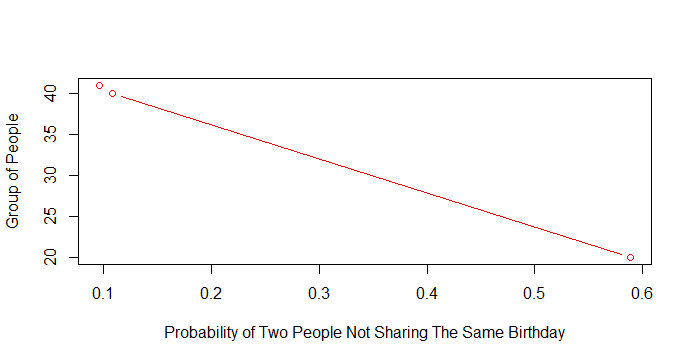
\includegraphics[scale=0.9]{fig1.1.png}
		\caption*{\footnotesize Plot 1.1 Examines how the probability of two people not sharing the same birthday is being influnced by the number of people in a group. See that as the number of people in a group rises the probability of two people not sharing the same birthday gradually decreases.}
		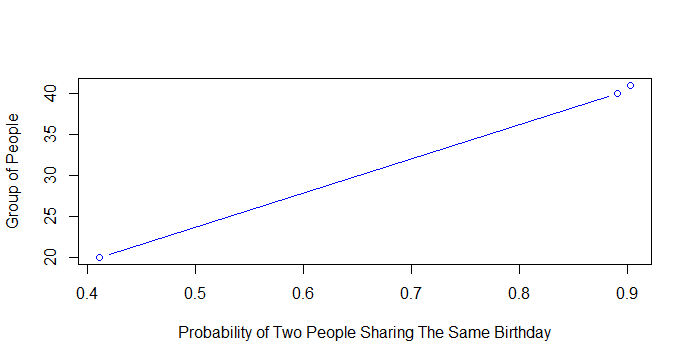
\includegraphics[scale=0.9]{fig1.2.png}
		\caption*{\footnotesize Plot 1.2 (above) Shows how the probability of two people sharing the same birthday is affected by the number of people in each group. As the number of people in a group increases the probability of two people sharing the same birthday also increases.}
	\end{figure}
	
	\pagebreak
	
\item \textbf{Mathematical Calculations}\\
	Even though we input this equation to a calculator because the chance is that it would display “Math Error” or “Syntax Error”, but to formality the equation we used to calculate the probability of two people sharing the same birthday is:
	
	\begin{equation*}
	\frac{364!}{365-n!}365^{n-1}
	\end{equation*}

Unfortunately, our calculator cannot perform such equation, so there’s no other choice but go on the long way; by multiplying the probability of two people not sharing the same birthday in a group of people (m) and the result is deducted to 1 to acquire the probability of two people sharing the same birthday in a group of people (n). \\\\
Since, $p(m) + p(n) =1$ then $p(n)= 1 -p(m)$\\
So, $p(m)=\frac{365}{365}\times\frac{364}{365}\times\frac{363}{365}\times\frac{362}{365}\ldots\frac{m}{365}$

\end{enumerate}

\pagebreak


%%%%%%%%%%%%%%%%%%%%%%%%%%%%%%%%%%%%%%%%%%%%%%%%%%%%%%%%%%%%%%%%%%%%%%%%%%%%%%%

\section*{PROBLEM 3}

\paragraph{\textbf{(COLOR GAME) } The color game is a popular betting game here in the Philippines. Three colored dice are being tossed and the player will bet money to one of the 6 colors. A player wins the same amount, twice the amount, or three times the amount of money he bet if the color he chose matches the colors from the 3 dice that has been rolled. Suppose that a player only bets one color for every round. Simulate this game and show that a player will eventually lose his money.}

\begin{enumerate}[label=\Alph*]
\item \textbf{Algorithm}

The game only allows the player to bet on a single color per round, this greatly reduces the probability of having a positive net money after playing the game. However, maximizing the chance of a player not losing all their money allows us to have a solid proof that they will indeed lose all of their money after enough rounds of playing the color game. To do this, we let them bet only a portion of their initial money for each `round; this amount can be obtained by multiplying their initial money by a betting percentage. Furthermore, since the exact color is not important, we represent the 6 colors using integers 0 to 5.

\begin{enumerate}
	\item[1] Input the initial money and the betting percentage per round. This parameter accepts floating-point values from 0 to 1. Additionally, a player can also input -1, this means that their betting percentage will be randomized every round.
	\item[2]\textit{Round start:} Add 1 to round counter. 
	\item[3] Calculate betting money by multiplying their balance with the betting percentage. Subtract the betting money from the balance. 
	\item[4] A color is randomly selected to be the bet color. 
	\item[5] \textit{Roll 3 dice:} A set of 3 colors are randomly chosen from a total of 18 (6*3) possible colors, each color is equally likely to be selected.
	\item[6] Count how many of the 3 rolled colors match the bet color. 
	\item[7] \textit{Compute winnings:} If there are matched colors, the bet money is doubled, tripled, or quadrupled, depending on the number of matched colors. The winnings will be added to the balance.
	\item[8] If the balance is non-zero, steps 2 to 8 are repeated. However, if the balance is 0, the game ends.
	\item[9] Return the game summary, where the trials and the player's betting money, chosen color, rolled colors, and match colors for each round are noted.
\end{enumerate}

\item \textbf{R Code}

\begin{lstlisting}[language=R]
#PARAMETERS: initial money of the player and the percentage of their money they are willing to bet. betting percentage can be -1, randomize betting percentage for every round
colorGame <- function(balance, betting_percentage){
  round <- 0 # store the number of rounds
  colors <- c(0:5) # represents the 6 colors per die
  chance <- c(rep(1/6, 6)) # probabilities of each color, future-proofed in case of biased die
  flag <- 0  # value of flag will be 1 if betting percentage is randomized, else 0
  if (betting_percentage==-1) flag <- 1
  
  set.seed(34029) # seed allows for replication of the same output
  gameSummary <- data.frame( # a blank data frame to tabulate the game summary
    Trial = integer(),
    Balance = integer(),
    Bet = integer(),
    Chosen_Color = integer(),
    Rolled_Colors = character(),
    Won = integer()) 
    
  repeat{ # loops until money is 0
    round <- round+1	# increment round counter
    if (flag==1) betting_percentage <- runif(1,min = 0, max=1.00001)    # randomize betting percentage if player decides to randomize
    
    # calculate betting money, subtracts it from the balance
    bet <- ceiling(balance*betting_percentage)
    balance <- balance-bet
    
    won <- 0  # variable to store the number of matched colors   
    betColor <- sample(colors, size = 1, prob = chance) # randomly choose a color among the 6 colors 
    rolledColor <- sample(colors, size = 3, prob = chance, replace=TRUE) # 1 color per die (3 dice in total) is randomly selected with replacement
    for(i in rolledColor)    # counts the number of winnings
      if (betColor == i) won <- won+1 
    gameSummary[nrow(gameSummary)+1,] <- c(round,balance,bet,betColor, toString(rolledColor),won)    # update gameSummary with new data from this round
    if (won>0) balance <- balance+(bet*(won+1))     # calculating the total money after the round 
    print(c(round,balance,bet,betColor, toString(rolledColor),won))    # for debugging purposes
    if (balance==0) break     # game ends, player loses since there is no money left
  }
  write.table(gameSummary, "gameSummary.csv", append=TRUE, sep=",", row.names = FALSE)  # write a csv file that records the information per round of the color game
  return (gameSummary)  # function returns a game summary where the necessary information about this game is tabulated
}

\end{lstlisting}


\item \textbf{Simulation and Analysis}\\
 Running the colorGame function with an arbitrary initial money of 10,000, a low betting percentage of 0.05, the color game ends after 1404 rounds, with a balance of 0 (Figure 2.1). If we run the game with the same initial money, but with a fairly high betting percentage of 0.90, the game ends after 7 rounds, and a balance of 0 (Figure 2.2). Additionally, if we run with the same betting percentages, but with a low initial money of 150, we get 626 rounds for the 0.05 (Figure 2.3), and only 4 rounds for the 0.90(Figure 2.4), both having 0 balance at the end. Due to the sheer number of rounds for these trials, a graph is used to visualize the balance per round.
\begin{figure}[H]
	\centering
	\begin{subfigure}[h]{0.4\textwidth}	
		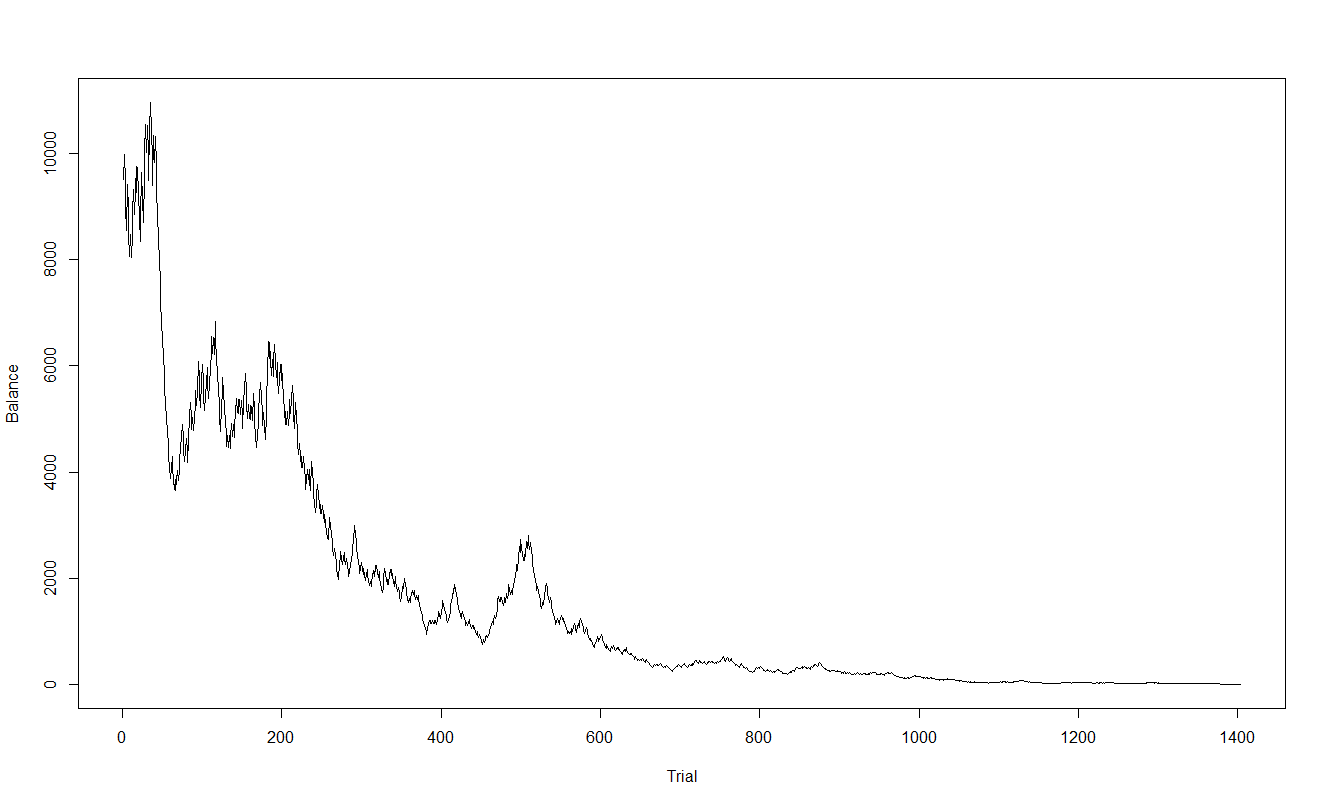
\includegraphics[width=\textwidth]{10000_0.05.png}
		\caption*{\footnotesize Figure 2.1 Graph of the simulation with initial money: 10,000, betting percentage:  0.05}
	\end{subfigure}~~~
	\begin{subfigure}[h]{0.4\textwidth}	
		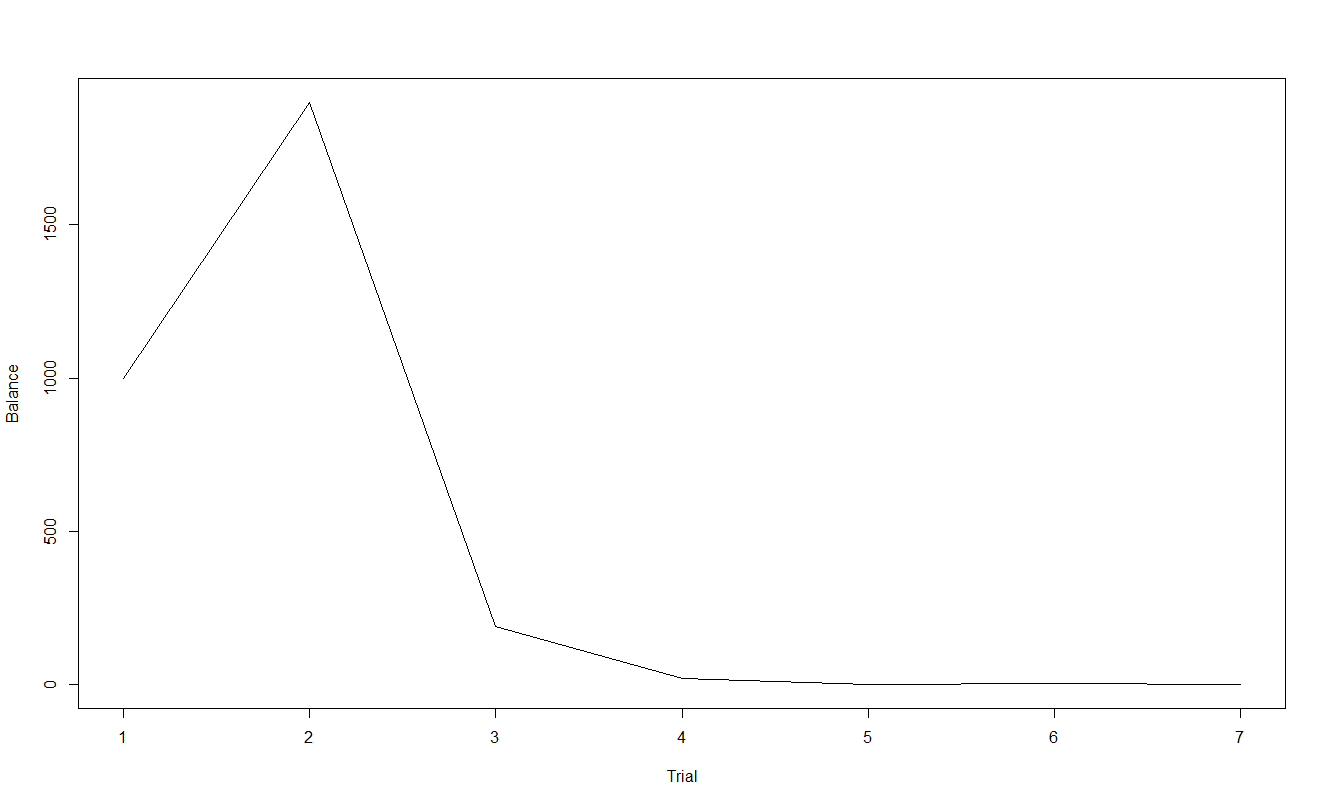
\includegraphics[width=\textwidth]{10000_0.9.png}
		\caption*{\footnotesize Figure 2.2 Graph of the simulation with initial money: 10,000, betting percentage:  0.90}
	\end{subfigure}
	
	\begin{subfigure}[H]{0.4\textwidth}	
		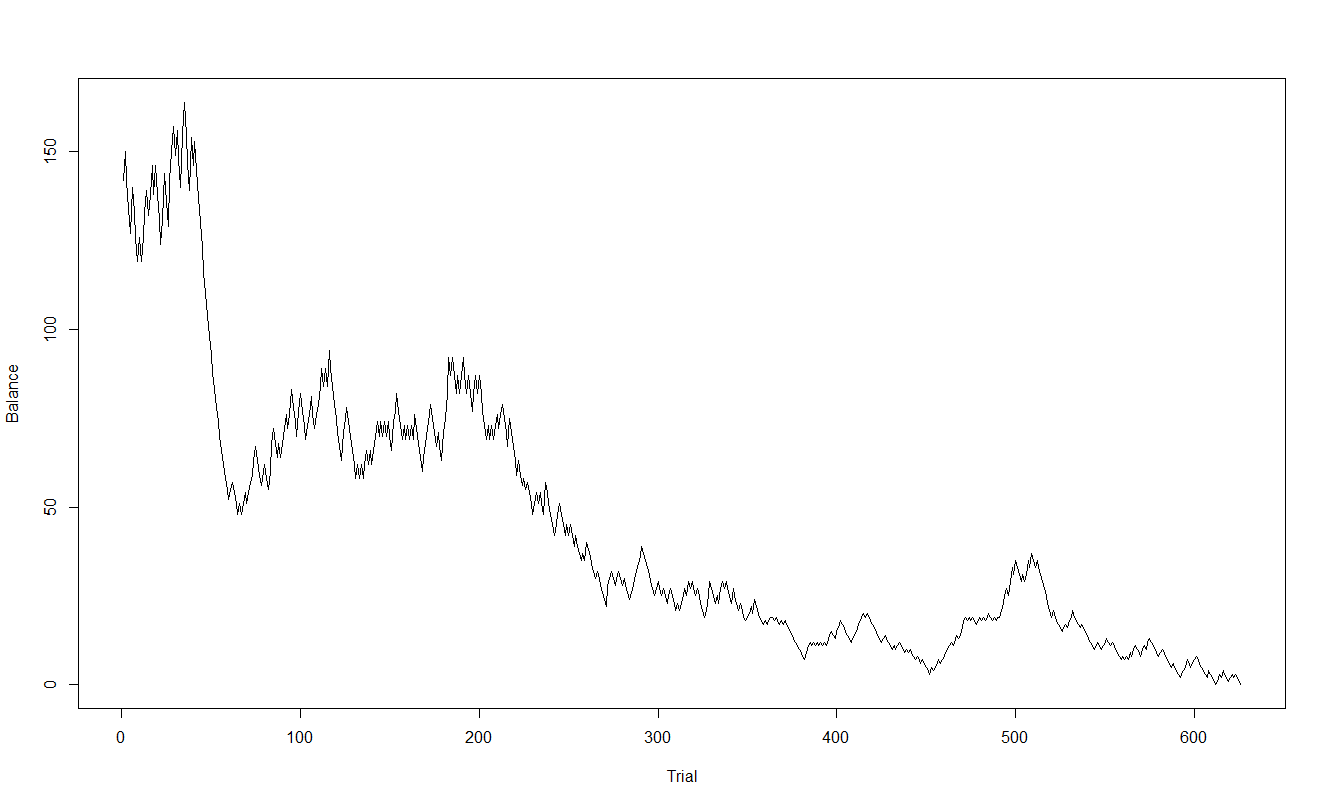
\includegraphics[width=\textwidth]{150_0.05.png}
		\caption*{\footnotesize Figure 2.3 Graph of the simulation with initial money: 150, betting percentage: 0.05}
	\end{subfigure}~~~
	\begin{subfigure}[H]{0.4\textwidth}	
		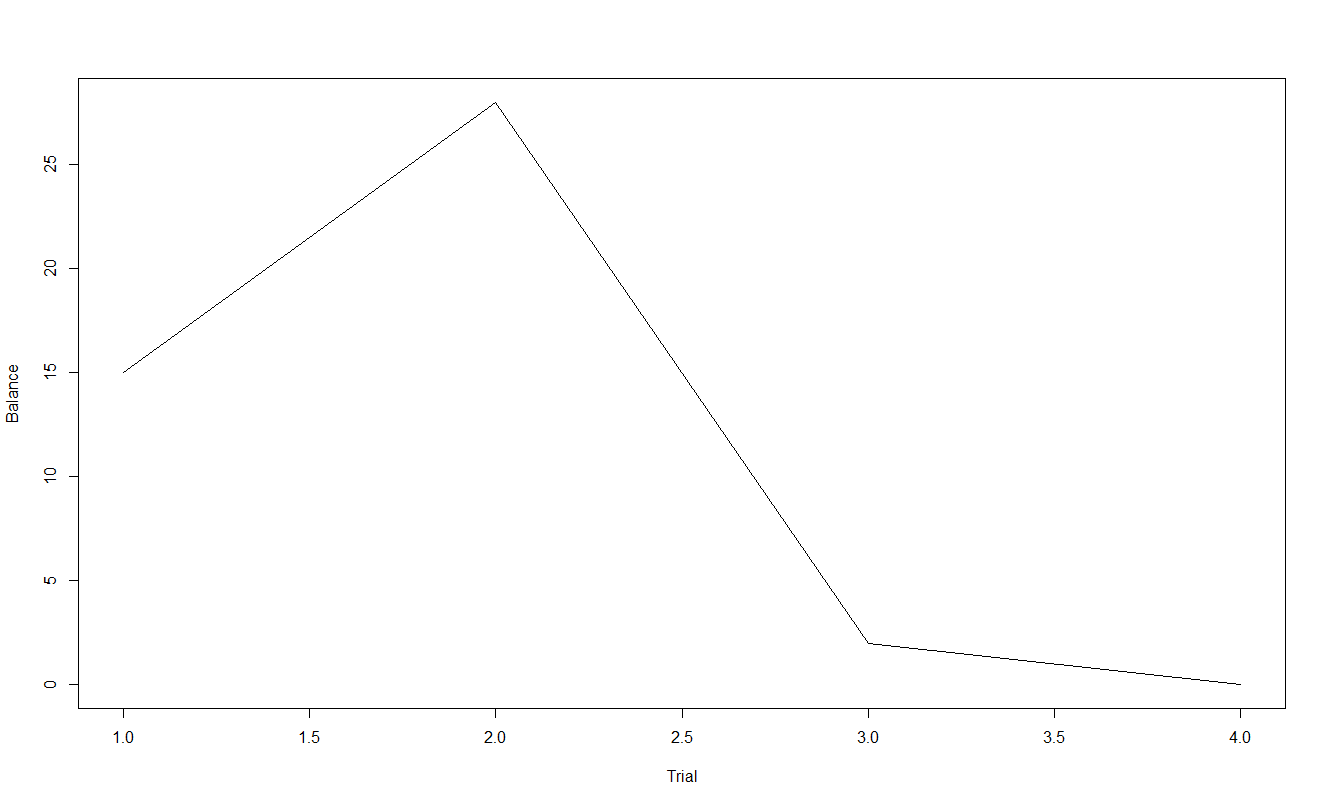
\includegraphics[width=\textwidth]{150_0.9.png}
		\caption*{\footnotesize Figure 2.4 Graph of the simulation with initial money: 150, betting percentage: 0.90}
	\end{subfigure}
\end{figure}


Although these 4 iterations of the color game showed the eventual loss of money, we still don't have enough confidence to conclude that the player will always lose their money. Thus, a second function is needed to replicate the color game as many as possible, with randomized initial money and betting percentages. The number of rounds it took for every iteration is also noted, to signify that the simulation really halted once the balance is 0.


\begin{lstlisting}[language=R]
#PARAMETERS: number of trials and the percentage of their money they are willing to bet. betting percentage can be -1, randomize betting percentage for every round
testColorGame <- function(trials, betting_percentage){
  
  set.seed(299792458) # seed allows for replication of the same output
  
  # a blank data frame to tabulate the results of the color game from randomized initial money
  testSummary = data.frame(
    Case = integer(),
    Money = integer(),
    Rounds = integer()) 
  
  for (i in 1:trials){ # loops until number of trials is reached
    
    # randomize the initial money using uniform distribution from 1 to 1,000,000
    money <- ceiling(runif(1,min=1,max=1000001)) 
    
    # get the number of rounds of this trial of color game from the game summary
    rounds <- nrow(colorGame(money, betting_percentage))
    
    #updates the table for this test
    testSummary[nrow(testSummary)+1,] <- c(i,money,rounds) 
  }
  
  # make a csv file to record results of the test
  write.table(testSummary, "testSummary.csv", append=FALSE, sep = ",", row.names = FALSE)
   
  # function returns a tabulated summary of this test, noting the initial money and the number of rounds it took to end the game
  return(testSummary)
}
\end{lstlisting}

Using the code above, the color game is repeated 100 times with randomized initial money (ranging from 1 to 1,000,000) and randomized betting percentages (from 0 to 1), using the code above. The results are presented in Table 2.1. Additionally, just to illustrate that having low betting percentages also lead to losing money, we simulate the game with a randomized betting percentage ranging from 0 to 0.25, see Table 2.2. With the 2 simulations, there is no doubt that the player will lose all their money after enough rounds of the color game, even though the second simulation took much longer than the first.\\

\begin{figure}[H]
\caption*{\footnotesize Table 2.1: Results of the simulated color game with 100 repetitions and randomized initial money and betting percentages}
	\small \centering
	\csvreader[tabular=lll,
	    table head=\hline Case & Money & Rounds\\\hline,
		table foot=\hline]
	{testColorGame_100_-1(0).csv}{}
	{\csvlinetotablerow}~~
	\csvreader[tabular=lll,
	    table head=\hline Case & Money & Rounds\\\hline,
		table foot=\hline]
	{testColorGame_100_-1(1).csv}{}
	{\csvlinetotablerow}~~
	\csvreader[tabular=lll,
	    table head=\hline Case & Money & Rounds\\\hline,
		table foot=\hline]
	{testColorGame_100_-1(2).csv}{}
	{\csvlinetotablerow}~~
	\csvreader[tabular=lll,
	    table head=\hline Case & Money & Rounds\\\hline,
		table foot=\hline]
	{testColorGame_100_-1(3).csv}{}
	{\csvlinetotablerow}%
\end{figure}

\begin{figure}[H]
\caption*{\footnotesize Table 2.2: Results of the simulated color game with 100 repetitions and randomized initial money and betting percentages ranging from 0 to 0.25}
\small \centering
	\csvreader[tabular=lll,
	    table head=\hline Case & Money & Rounds\\\hline,
		table foot=\hline]
	{testColorGame_100_0-0.25(0).csv}{}
	{\csvlinetotablerow}~~
	\csvreader[tabular=lll,
	    table head=\hline Case & Money & Rounds\\\hline,
		table foot=\hline]
	{testColorGame_100_0-0.25(1).csv}{}
	{\csvlinetotablerow}~~
	\csvreader[tabular=lll,
	    table head=\hline Case & Money & Rounds\\\hline,
		table foot=\hline]
	{testColorGame_100_0-0.25(2).csv}{}
	{\csvlinetotablerow}~~
	\csvreader[tabular=lll,
	    table head=\hline Case & Money & Rounds\\\hline,
		table foot=\hline]
	{testColorGame_100_0-0.25(3).csv}{}
	{\csvlinetotablerow}%
\end{figure}

\pagebreak

\end{enumerate}

%%%%%%%%%%%%%%%%%%%%%%%%%%%%%%%%%%%%%%%%%%%%%%%%%%%%%%%%%%%%%%%%%%%%%%%%%%%%%%%%%%%%%%%

\section*{PROBLEM 4}

\paragraph{(THE POWER SET) A collection of all possible subsets $\{E_{i}\}\in\omega $ is called the \textit{power set} of $\Omega$, denoted by $\rho(\Omega)$. For example, if $\Omega=\{1,2,3\}$, then its power set is given by $\rho(\Omega)=\{\emptyset,\Omega, \{1\}, \{2\}, \{3\} \}, \{1,2,\}, \{1,3\}, \{2,3\}$. Note that all power sets are valid event spaces.}

\begin{enumerate}
\item[(a)] Create a function that generates the power set of any given vector.
\item[(b)] Create another function that validates whether the generated power set is an event space
\end{enumerate}

\begin{enumerate}[label=\Alph*]
\item \textbf{R Code and Analysis}

(A) Create a function that generates the power set of any given vector
\begin{lstlisting}[language=R]
#A)Create a function that generates the power set of any given vector.
powerSet <-function (x, m, rev = FALSE) 
{
  if (missing(m)) m = length(x)
  if (m == 0) return(list(x[c()]))
  
  out = list(x[c()])
  if (length(x) == 1) 
    return(c(out, list(x)))
  for (i in seq_along(x)) {
    if (rev) 
      out = c(lapply(out[lengths(out) < m], function(y) c(y, x[i])), out)
    else out = c(out, lapply(out[lengths(out) < m], function(y) c(y, x[i])))
  }
  out
}
\end{lstlisting}

\textbf{RECALL,}\\
\textbf{Power Set} Power set $\mathcal\{P\}(S)$ of a set S is the set of all subsets of S. For example $S = \{a, b, c\}$ then $\mathcal{P}(s) = \{\{\emptyset\}, \{a\}, \{b\}, \{c\}, \{a, b\}, \{a, c\}, \{b, c\}, \{a, b, c\}\}$. If S has n elements in it then $\mathcal{P}(s)$ will have $2^n$ elements.\\\\
The powerSet function produces the power set of a vector. \\
Creates a list containing every subset of the elements of the vector $\backslash code\{x\}$.\\
$\bullet$ parameter x, vector of elements (the set).\\
$\bullet$ parameter m, maximum cardinality of subsets.\\
$\bullet$ parameter rev, logical indicating whether to reverse the order of subsets.\\

It first checks the parameters defined or inputted. It is composed of if, if-else statements and a recursive function that passes each argument to a certain output for a condition that it satisfies. In the first if statement, if there is no maximum cardinality of subsets that is inputted, then it returns an empty/null set. In the next if statement, it checks the vector of elements. Last is the recursive function that outputs the order of the subsets of the power set.


\begin{center}
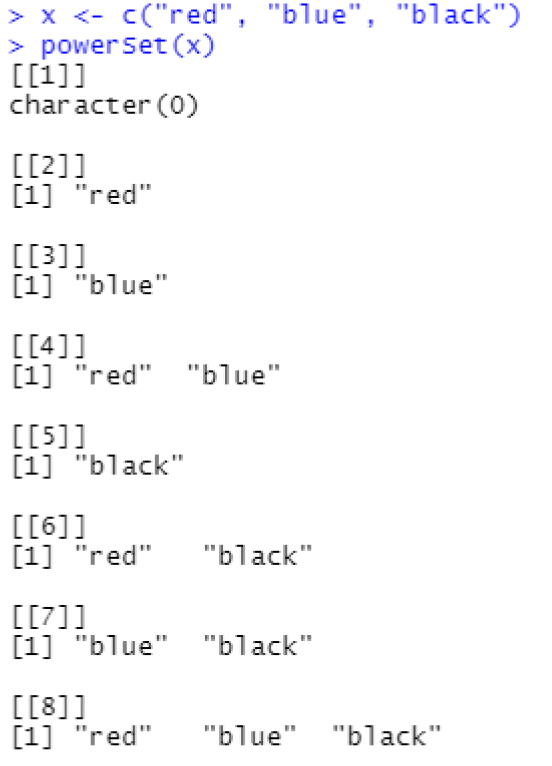
\includegraphics[scale=0.4]{fig4.1}\\
\textit{\footnotesize OUTPUT: power set of set $(x) = \{red, blue, black\}$}
\end{center}  

(B) Create another function that validates whether the generated power set is an event space.
\begin{lstlisting}[language=R]
B)Create another function that validates whether the generated power set is an event space.
validate <- function(powerSet){

  x <- c("1", "2", "3")
  
  #defining the possible outputs
  valid <- ("VALID. The power set is an event space.")
  invalid <- ("INVALID. The power set is not an event space.")
  
  n <- length(x)
  cardinality <- length(powerSet)
  
  #if/else function to identify whether the power set is an event space
  if(2^n != cardinality){
    return(valid)
  }else {
    return(invalid)
  }
}
\end{lstlisting}

\textbf{RECALL,}\\
\textbf{Power Set} Power set $\mathcal\{P\}(S)$ of a set S is the set of all subsets of S. For example $S = \{a, b, c\}$ then $\mathcal{P}(s) = \{\{\emptyset\}, \{a\}, \{b\}, \{c\}, \{a, b\}, \{a, c\}, \{b, c\}, \{a, b, c\}\}$. If S has n elements in it then $\mathcal{P}(s)$ will have $2^n$ elements.\\\\
\textbf{Cardinality} is the number of elements of the set.\\\\
The validate function validates if the generated power set is a valid event space or not. For the power set to be a valid event space, it must have the right cardinality of elements. This function contains an if-else statement that checks the cardinality of elements within the power set and returns VALID and INVALID as its outcomes. If the defined set has $2^n$ elements, then it is a valid event space. Otherwise, it is invalid.

\begin{center}
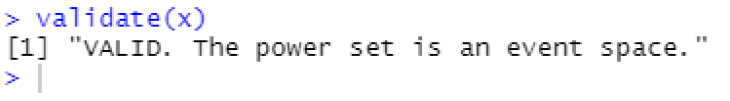
\includegraphics[scale=0.4]{fig4.2}\\
\textit{\footnotesize OUTPUT: The defined set $(x)= \{red, blue, black\}$ is a VALID event space since it has $2^n$ cardinality of elements.}
\end{center}  
\end{enumerate}


\pagebreak

%%%%%%%%%%%%%%%%%%%%%%%%%%%%%%%%%%%%%%%%%%%%%%%%%%%%%%%%%%%%%%%%%%%%%%%%%%%%%%%%%%%%%%%%%%%%%%%%%%%
\section*{PROBLEM 5}

\paragraph{(A KNIGHT'S TALE) Using brute force, find the minimum number of moves a horse can make to cover all the tiles in a chess board. The starting point of the horse should only be one of the 4 corner tiles}

\begin{enumerate}[label=\Alph*]

\item \textbf{Algorithn and R Code}

The board is created as a 8x8 matrix with -1 as its initial value. 
\begin{lstlisting}[language=R]
board = matrix(-1, nrow = 8, ncol = 8)
\end{lstlisting}

Then there are two functions to update and get information about the board, get\_board and set\_board.
\begin{lstlisting}[language=R]
set_board = function(x,y,move){board[x,y] <<- move}
get_board = function(x,y){board[x,y]}
\end{lstlisting}

Get\_board returns a value of the board in the position, while set\_board on the other hand sets a value in that position.
\begin{lstlisting}[language=R]
x_move = c(2,1,-1,-2,-2,-1,1,2)
y_move = c(1,2,2,1,-1,-2,-2,-1)
\end{lstlisting}

The x\_move and the y\_move are two vectors or arrays that dictates the movement behavior of the knight.
\begin{lstlisting}[language=R]
valid_move = function(x,y){
  if(x >= 1 & x <= 8 & y >= 1 & y <= 8){
    return (get_board(x,y) == -1)
  }
  return (FALSE)
}
\end{lstlisting}

The valid\_move function checks if the position of the knight moves is valid or not and returns a boolean value in return.
\begin{lstlisting}[language=R]
knight_move = function(move, x, y){
  if(move == 64){
    return (TRUE)
  }
  
  for(i in 1:8){
    next_x = x + x_move[i]
    next_y = y + y_move[i]
    
    if(valid_move(next_x,next_y)){
      print(board)
      set_board(next_x,next_y,move)
      if(knight_move(move + 1, next_x, next_y)){
        return (TRUE)
      }
      else{
        set_board(next_x,next_y,-1)
      }
    }
  }
  return (FALSE)
}
\end{lstlisting}

The knight move is the function that records how many times the knight moves and as to what position the knight will move. It first checks if the total moves is 64 which is the maximum amount the knight can move which means covering all squares or positions in the board. Then the program goes to a for loop where it moves the knight downward then right in a counterclockwise movement. The program runs recursively which means it calls itself and checks all possible locations and if a route is to be found not the viable option then the program backtracks until it found another possible route to take on to. If the route ends and it did not cover the whole board then it returns FALSE and changes the value of that position to -1 then backtracks. If it is the solution then it returns TRUE.

\begin{center}
\centering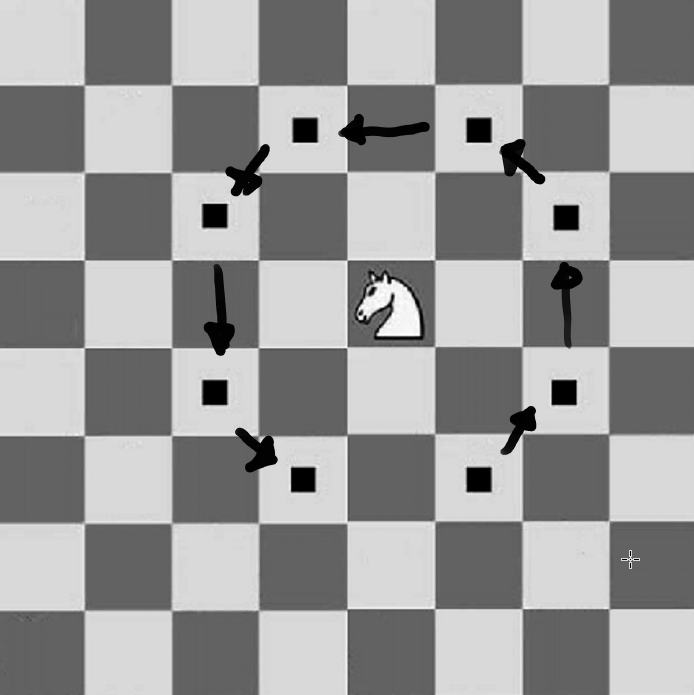
\includegraphics[scale=0.4]{number 5.png}
\end{center}

The solve function is the one that calls the knight\_move function and checks if the
problem can be solved or not, and if not, then it prints the board and “No route is true”.
\begin{lstlisting}[language=R]
solve = function(){
  set_board(1,1,0)
  if(knight_move(1,1,1)){
    print(board)
  }
  else{
    print(board)
    print("NO ROUTE IS TRUE")
  }
}
\end{lstlisting}
\pagebreak
\item \textbf{Simulation}\\
For the solution, the problem has a route and a solution. The problem can be solved
having a total move of 64 moves, starting at 0 up to 63.

\begin{table}[H]\centering
	\begin{tabular}{@{}l|llllllll@{}}
		\toprule
		       & [,1] & [,2] & [,3] & [,4] & [,5] & [,6] & [,7] & [,8] \\ \midrule
		$[1,]$ & 0 	  & 59   & 38   & 33   & 30  & 17    & 8    & 63   \\
		$[2,]$ & 37   & 34   & 31   & 60   & 9   & 62    & 29   & 16   \\
		$[3,]$ & 58   & 1    & 36   & 39   & 32  & 27    & 18   & 7    \\
		$[4,]$ & 35   & 48   & 41   & 26   & 61  & 10    & 15   & 28   \\
		$[5,]$ & 42   & 57   & 2    & 49   & 40  & 36    & 6    & 19   \\
		$[6,]$ & 47   & 50   & 45   & 54   & 25  & 20    & 11   & 14   \\
		$[7,]$ & 56   & 43   & 52   & 3    & 22  & 13    & 24   & 5    \\
		$[8,]$ & 51   & 46   & 55   & 44   & 53  & 4     & 21   & 12   \\ \bottomrule
	\end{tabular}
\end{table}

\end{enumerate}

\end{document}